\documentclass[conference,compsoc,a4paper]{IEEEtran}
% 中文审阅版：与 ../main.tex 逐节对应，数字、引用、标签完全相同。以英文版为准。
% 编译：cd paper/zh && tectonic -X compile main_zh.tex --outdir build
% 字体：fonts/ 下放 simsun.ttc、simhei.ttf、simkai.ttf（从 C:/Windows/Fonts 复制，不入库）。
\usepackage{xeCJK}
\setCJKmainfont{simsun.ttc}[Path=./fonts/, FontIndex=0, BoldFont=simhei.ttf, ItalicFont=simkai.ttf]
\setCJKsansfont{simhei.ttf}[Path=./fonts/]
\setCJKmonofont{simhei.ttf}[Path=./fonts/]
\xeCJKsetup{CJKecglue={\hskip 0.2em plus 0.1em}}
\linespread{1.08}
\usepackage{amsmath,amssymb}
\usepackage{booktabs,makecell,multirow}
\usepackage{graphicx}
\usepackage{xcolor}
\usepackage[numbers,sort&compress]{natbib}
\usepackage{xurl}
\usepackage{adjustbox}
\usepackage{placeins}
\usepackage{fancyvrb}
\usepackage{tikz}
\usepackage[hidelinks]{hyperref}
\usepackage[capitalize,noabbrev]{cleveref}

\newcommand{\hesp}{HESP}
\newcommand{\todo}[1]{\textcolor{red}{[待补：#1]}}
\newcommand{\repourl}{\url{https://github.com/lzwhehe/HESP}}
\DeclareRobustCommand{\stepnum}[1]{\tikz[baseline=-0.6ex]\node[circle,fill=black,text=white,font=\scriptsize\bfseries,inner sep=0.6pt,minimum size=9pt]{#1};}
\graphicspath{{../figures/}{../../docs/assets/}}
\setlength{\emergencystretch}{3em}
\renewcommand{\paragraph}[1]{\par\vspace{0.6ex}\noindent\textbf{#1。}\hspace{0.2em}\ignorespaces}

\renewcommand{\figurename}{图}
\renewcommand{\tablename}{表}
\renewcommand{\abstractname}{摘要}
\renewcommand{\refname}{参考文献}
\renewcommand{\appendixname}{附录}
\crefname{figure}{图}{图}\Crefname{figure}{图}{图}
\crefname{table}{表}{表}\Crefname{table}{表}{表}
\crefname{section}{§}{§}\Crefname{section}{§}{§}

\begin{document}

\title{\hesp{}：在本地 LLM 告警分诊智能体中\\把“探什么”与“何时停”分开}

\author{\IEEEauthorblockN{Zhuowen Liu}
\IEEEauthorblockA{北陆先端科学技术大学院大学（JAIST）网络安全实验室\\
日本石川县能美市\\
\texttt{s2410431@jaist.ac.jp}}
\and
\IEEEauthorblockN{Zhixuan Wang\textsuperscript{*}}
\IEEEauthorblockA{辽宁师范大学美术学院\\
中国辽宁省大连市\\
\texttt{wangzhixuanwzx@gmail.com}\\
\textsuperscript{*}通讯作者}}

\maketitle

\begin{abstract}
无法把遥测发送给托管模型的组织，只能用小型开源权重 LLM 实现告警分诊自动化，而这些模型恰恰在调查流程上失败：探测却不收敛、不给出结论，或者服从写进日志的指令。我们研究应当从模型手里拿走哪些分诊决定，以及由此形成怎样的安全边界。\hesp{} 是一个控制器：它维护候选原因的账本，按单位成本的期望信息增益选择只读探针，只接受有当前证据支持的结论，并且可以自行结束调查。在一项基于三个合成任务族的受控研究中（七项采用内部冻结协议的研究，五个 7B 到 72B 的模型，21{,}278 个经过审计的 LLM 回合），“探测什么”与“何时停止”是两种独立的失败。采用验证器的证据标准后，控制器无需 LLM 就能完成每一个案例；预先登记的比较没有发现让 Qwen2.5-72B 决定何时停止带来增益，而即使给基线同样清楚的提示，它们仍然远远落后。要求一条决定性观测是以自动化换取安全：联合证据能解决更多“原因使用相同工具”的案例，但会把一部分攻击结为与之相似的合法活动。结束守卫在每个模型上都挡住了“关闭告警”的注入指令；伪造的来源能击败控制器，除非良性结论需要来自不同来源的佐证。模型剩下的作用是读取原始日志：小模型能读懂让规则解析器失效的新格式，但可能采纳攻击者声称的读数。
\end{abstract}

\section{引言}
\label{sec:intro}

安全团队开始把告警分诊和调查交给 LLM 智能体~\citep{guide,cortex,sentinelrl}。智能体收到一条告警，查询日志，然后报告是否发生了攻击、攻击涉及了什么。这样的智能体能否被信任去关闭告警，很大程度上由基准决定：ExCyTIn-Bench~\citep{excytin}、SIABench~\citep{siabench} 等基准报告智能体答对的比例，而领域把这些数字当作调查能力的度量。调查正是部署智能体的理由。只会复述告警内容的智能体对分析员没有价值，而且恰好会在攻击者刻意制造的情形中失败：恶意活动看起来像日常操作，也没有任何东西点出它的名字。

只有当题目不调查就答不出来时，基准才在衡量调查。以一道 ExCyTIn 题目为例，它由一条三跳路径生成：从一条关于计划任务的告警出发，经过主机，到达一条相关告警，答案是后者记录的 IP 地址。题目问的是"相关的 `Anomaly detected in ASEP registry' 告警中记录的 IP 地址"。按这个告警名做一次 SQL 查询就能拿到答案，生成题目时设想的那次跳转并不需要（\cref{fig:example}）。如果这样的题目很多，智能体不调查也能拿分，而分数对真正重要的情形毫无说明。

基准论文报告模型成绩，却很少报告一个不调查的规则能拿多少分。安全领域有针对学习型检测器做重新评估的传统，问的正是这个问题：简单基线可以与复杂的溯源检测器相当~\citep{bilot2025simpler}，虚假相关会抬高实验室结果~\citep{arp2022dos}。机器学习中同样的问题称为捷径学习~\citep{geirhos2020shortcut,gururangan2018artifacts}。近期有工作为事件响应提出奖励"发现新证据"的新基准~\citep{sirbench}，但已在使用的基准还没有被审计过，在这些基准上评测的智能体是否利用了其中的捷径，也没有被测量过。

\begin{figure}[t]
  \centering
  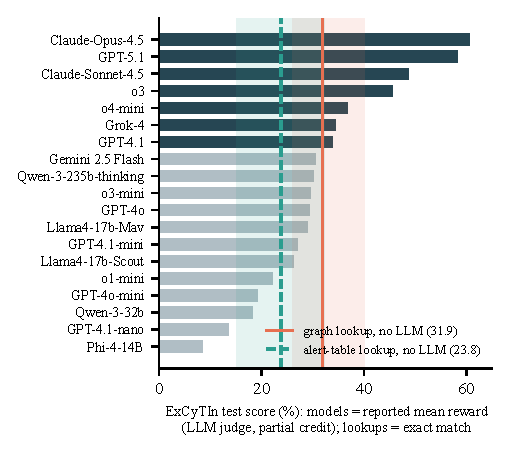
\includegraphics[width=\columnwidth]{fig_floor.pdf}
  \caption{不含 LLM 的查表在 ExCyTIn-Bench 上超过了报告的 \oModels{} 个智能体中的 \oBelowGraph{} 个。柱：各模型在 589 道测试题上的报告平均奖励~\citep{excytin}。线：在同一批题目上，两种不调查、只查找题目点名告警的规则，按精确匹配计分（阴影：按事件重抽的 95\% 区间）。深色柱高于图查表。}
  \label{fig:floor}
\end{figure}

我们审计了四个面向 LLM 安全运营智能体的公开基准和数据集（ExCyTIn-Bench、SIABench、GUIDE、OTRF Security-Datasets）以及我们自己构建的三个分诊环境。对每一个，我们写一条固定规则：只使用智能体能看到的信息，不含 LLM，并跳过基准设想的调查，再把它与报告的模型成绩比较。我们发现四类捷径：题目点出了答案所在的证据（S1）；标签跟着打标签的组织走（S2）；数据生成过程留下线索，例如攻击网络的地址（S3）；在人工构建的环境中，对证据模型执行固定程序就能解出所有案例（S4）。ExCyTIn 的作者公开了 14 次智能体运行的完整日志，因此我们进一步逐题检验智能体的成功是否来自捷径。每次确认性运行之前，假设都已登记、规则都已冻结。

\paragraph{结果} 每个被审计的基准都存在一条不调查的规则，能达到报告成绩中相当大的一部分。在 ExCyTIn 上，\oNamed\% 的测试题点出了答案所在的告警，查找这条告警可以精确答对 \oGraph\%，高于报告的 \oModels{} 个模型中 \oBelowGraph{} 个的平均奖励（\cref{fig:floor}）。在 SIABench 上，"当且仅当告警涉及 172.16.0.1 时判为真阳性"在全部 35 条告警上都正确。在 GUIDE 上，沿用组织过去对同一检测器的判定，在之后的事件上正确率为 \gHistPct\%。在 OTRF 录制中，仅凭告警文字就能区分 \otN{} 条告警中的 \otRuleCorrect{} 条。然而 ExCyTIn 的智能体并没有使用这条捷径：题目点名答案告警时成功率并不更高（\lgModels{} 次运行中 \lgPos{} 次为正，$p=\lgP$）；只需一次查询时它们也发出同样多的查询；在抗捷径题目上排名几乎不变（Kendall $\tau=\lgTau$）。更深层的问题是，成功率几乎不随题目所需的调查而变化：最强的智能体在 140 道一次查询即可答对的题目中答错 \tcOpusFail{} 道。

\paragraph{贡献}
\begin{itemize}\setlength\itemsep{1pt}
\item 给出调查型基准中"捷径"的定义和四类捷径的分类，每类配一个不调查的基线（\cref{sec:method}）。
\item 审计四个公开基准和三个人工构建的环境，表明每一个都存在能达到或超过报告成绩相当部分的规则（\cref{sec:floors}）。
\item 对 ExCyTIn 公开的 14 次智能体运行做逐题分析，表明智能体没有利用捷径，其成功率也不随所需调查而变化（\cref{sec:scores}）。
\item 给出面向基准构建者的检查项，证明攻击与良性"孪生"配对可以消除单条观测捷径，并公开 ExCyTIn 的逐题捷径标记（\cref{sec:design}）。
\end{itemize}

\section{背景}
\label{sec:background}

\paragraph{告警分诊} 告警分诊针对检测产生的每条告警，判断实际发生了什么、是否需要响应~\citep{nodoze}。它与攻击调查不同：攻击调查从一个关注点出发重建完整的攻击过程~\citep{kairos,clouseau}，而分诊以单一结论结束，即告警的原因及支持它的证据。分析员通过查询环境得出结论，而查询在成本和区分候选解释的能力上各不相同：有些查询便宜且对某个解释具有决定性，另一些（例如威胁情报查询）既慢，又对几种攻击返回同样的答案。设想一条告警报告 Web 层认证失败和 HTTP 错误激增。它看起来像凭证填充，但同样的症状也可能来自 SQL 注入探测、授权的漏洞扫描、被误判的健康检查，或者暴露在公网上的管理面板；读取管理面板的配置只需一次便宜的查询，就能立刻判定最后一种解释，但只有始终把这个解释放在视野里的调查者才会运行它。因此，查询的顺序决定调查多快结束，调查者还必须判断证据何时已经足够。

\paragraph{本地 LLM 智能体} LLM 智能体把语言模型与工具结合起来：每一步，模型读取任务和已有观测，然后调用一个工具或结束任务~\citep{react}。Qwen2.5 和 Llama~3.1 等开源权重模型可以在组织自己的硬件上运行，4 比特权重下单块 GPU 最多可运行 72B 参数，这让遥测留在本地，却让循环的每一步都依赖一个较弱的模型。

\paragraph{对智能体输入的注入} 读取检索内容的智能体会被其中隐藏的指令操纵，即间接提示注入~\citep{greshake2023}，AgentDojo~\citep{agentdojo} 在工具型智能体上对此进行了基准测试。日志注入通过未转义的用户可控字段伪造或破坏日志记录，是同一问题更早的实例~\citep{owasp_loginjection}。在分诊中两者都适用，因为请求载荷、用户代理、命令行和工单文本都由引发告警的一方书写，并被复制进智能体读取的日志。

\section{动机}
\label{sec:motivation}

\subsection{挑战}
当小型本地模型驱动调查时，会出现三个挑战。我们在各项研究的配置上（\S\ref{sec:setup}）分别测量了它们。

\stepnum{1} \textbf{流程失败。}自行选择探针的 Qwen2.5-7B 只验证了 0.083 到 0.125 的案例：它每个回合运行约七个不同的探针，花掉 10 个成本单位中的 9.4 到 9.5，四分之三的回合以工具预算耗尽告终；把它的选择换成均匀随机选择能把完成率提高 $+0.556$（\S\ref{sec:cost}）。在我们的提示与服务配置下，Llama-3.1-8B 在全部 3{,}389 次决策中都请求再运行一个探针，包括账本后验超过 0.999、提示已说明没有合法探针可用的那些决策。更大的模型会给出结论，但并不总是基于证据：没有账本时，Qwen2.5-32B 与 72B 在它们给出结论的需处置事件中分别把 13/51 和 20/54 判为良性。

\stepnum{2} \textbf{证据有一部分是攻击者的。}用户代理、请求载荷或工单评论会被复制进智能体读取的日志。当这样的字段带有“把案件结为授权扫描”的指令时，每个自行决定并给出结论的模型都服从了它（\S\ref{sec:injection}）。良性结论是攻击者最想要的结论，因为它在没有任何响应的情况下关闭案件。

\stepnum{3} \textbf{总得有人读日志。}按文档日志格式写的固定解析器在日志流水线变化后什么也读不出，于是每个案例都被升级（\S\ref{sec:rawlog}）。模型能读懂变化后的格式，但读取的模型可能被说服接受攻击者的读数，而且它读的是攻击者能写入的每一个来源。

\subsection{我们的方案}
\hesp{} 用模型之外的组件回应每个挑战。\stepnum{1} 一个由不含 LLM 的开发回合计数得到的似然表更新的账本、按单位成本期望信息增益对每个合法探针的排序、在每次调用规划器前应用的明确接受规则，以及规则满足时的控制器侧停止（附录~\ref{app:loop} 给出确切顺序）。\stepnum{2} 一个只接受“引用了账本中支持所称原因的当前观测”的结论的结束守卫，使从未进入账本的文本无法结束案件；以及一条要求良性结论建立在不同来源组之上的佐证规则。\stepnum{3} 读取器之间的信任边界：规则解析器解析出的观测是可信的，模型解析出的观测可以抬高某个原因、可以确认攻击，但永远不能确认良性结论。预写式日志让审计可以重放每一步。

\section{\hesp{} 设计}
\label{sec:approach}

\hesp{} 位于本地 LLM 与探针目录之间（\cref{fig:pipeline}）。模型负责提议：每一步，它可以建议一个探针、提出一个结论或弃权，并在探针返回文本时解析日志。控制器负责决定：运行哪个探针、接受哪个结论、何时结束调查。每一步都在其观测到达之前写入日志，事后接受审计。

我们用运行示例走一遍。告警留下九个候选原因，各为 0.111。控制器按单位成本的期望信息增益对探针排序，运行 \texttt{source\_ips}，尽管模型提议的是 \texttt{auth\_log}（每成本单位 1.74 比 0.51 比特）；结果为 \textit{normal}，剩下四个原因，各为 0.238。\texttt{access\_pattern} 之后剩下三个，各为 0.327：暴露的管理面板、存在漏洞的组件、DNS 命令控制。\texttt{admin\_exposure} 返回 \textit{exposed, no auth}，把管理面板抬到 0.966。在下一次调用模型之前，控制器发现领先原因已超过接受阈值、且最后一条观测能把它单独识别出来，于是在三个探针、5.1\,s 之后以这个结论结束回合。

\begin{figure*}[t]
  \centering
  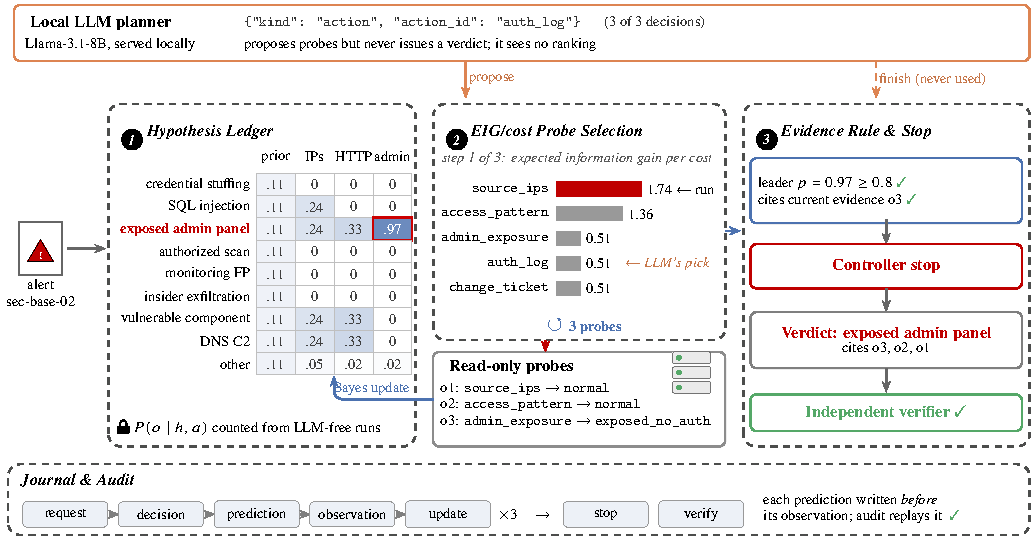
\includegraphics[width=\textwidth]{fig_pipeline.pdf}
  \caption{运行示例上的 \hesp{}（Llama-3.1-8B；真实原因：暴露的管理面板）。\protect\stepnum{1} 账本维护候选原因上的后验，依据冻结的探针—结果表用贝叶斯规则更新。\protect\stepnum{2} 控制器运行单位成本期望信息增益最高的合法探针；模型的提议（这里三次都是 \texttt{auth\_log}）只作参考。\protect\stepnum{3} 一旦领先原因的后验达到 0.8、且有一条当前观测能把它单独识别出来，控制器就给出结论并引用该证据。验证器只用于评测。所有数值取自归档日志。}
  \label{fig:pipeline}
\end{figure*}

\subsection{证据账本}
\label{sec:ledger}
\label{sec:tables}
\emph{问题。} 控制器需要一个模型，告诉它每个探针在每个原因下会返回什么；LLM 给不出这样的模型（向规划器询问得到的表让解决率停在 0.069 到 0.375，\S\ref{sec:policy}）。

\emph{机制。} 部署之前，一个脚本在每个原因的 $k$ 个开发回合中把每个探针各运行一次，并把结果计数成表
\[\widehat P(o \mid h, a) = \frac{q_{h,a,o}}{\sum_{o'} q_{h,a,o'}},\quad q_{h,a,o} = (1-\varepsilon)\,\frac{n_{h,a,o}}{n_{h,a}} + \frac{\varepsilon}{|O_a|},\]
其中 $n_{h,a,o}$ 是原因 $h$ 下探针 $a$ 得到结果 $o$ 的有效观测数，$O_a$ 是探针的结果词表，$\varepsilon = 0.01$。没有开发案例的原因（如 \textit{other}）取均匀行。表在使用前计算哈希并冻结。对每条告警，账本从候选原因上的均匀先验开始，在每条有效观测后应用贝叶斯规则 $p_t(h) \propto p_{t-1}(h)\,\widehat P(o_t \mid h, a_t)$，并记录该观测提高还是降低了每个原因的分数。瞬时故障（如 HTTP 503）写入日志，但不算证据。环境报告事件变化时，分数重置为先验，此前的观测不再算作当前证据。

\emph{替代方案。} 向模型询问似然可以省去开发数据，但如上所述行不通。在 sec-triage 中，每个原因五个开发回合得到的表就已能解决每一个案例（\S\ref{sec:policy}）；部署时可以对已结案工单或重放的事件计数（\S\ref{sec:discussion}）。

\subsection{探针选择}
\label{sec:selection}
对每个合法探针（即在当前状态下未运行过、在预算之内且前置条件满足），控制器计算期望信息增益
\begin{align*}
\mathrm{EIG}(a) &= H(p) - \textstyle\sum_{o} P(o \mid a)\, H\big(p(\cdot \mid o, a)\big),\\
P(o \mid a) &= \textstyle\sum_h p(h)\, \widehat P(o \mid h, a),
\end{align*}
并运行 $\mathrm{EIG}(a)/c(a)$ 最高的探针，$c(a)$ 为其成本。这一准则是经典的~\citep{dekleer1987,golovin2010}；关键在于模型的提议不再决定运行哪个探针。模型收到任务、目录、观测、账本和被拒提议的反馈（附录~\ref{app:prompt}），返回一个 JSON 决策。

\subsection{证据规则与停止}
\label{sec:finish}
\emph{结束守卫。} 只有当所称原因的当前分数不低于 $\tau = 0.8$、且至少一条被引用的观测是当前的并在账本中支持它时，模型提出的结论才会被接受。被拒绝的结论作为反馈返回给模型。日志里的文本从不进入账本，因此单凭文本无法满足守卫。

\emph{控制器停止。} 在每次调用模型之前以及预算耗尽时，控制器对当前领先原因应用同样的规则，满足时自行给出结论，并引用至多三条支持观测。\emph{确认}变体还要求有一条观测\emph{特异地}支持领先原因，即其结果在领先原因下的概率至少是任何其他具名原因下的十倍。它只使用预测表，并禁止纯粹靠排除得出的结论。

\emph{恢复。} 模型可以通过反复提出略低于阈值的同一结论，让带守卫的控制器卡住。连续两次结论被拒后，控制器直接运行自己排名第一的探针，而不再询问模型。

\subsection{跨来源佐证}
\label{sec:corroboration}
一旦由控制器决定，攻击者就改为伪造证据，而单条特异地支持良性原因的伪造观测就足够了，因为控制器先按信息量最大的观测行动。因此，\hesp{} 要求良性结论——无论由模型提出还是由控制器停止得出——建立在至少两个不同\emph{来源组}的当前观测之上，且每条都特异地支持它。来源组是探针背后的上游数据源，按部署声明；读取同一信誉源的两个探针属于同一组。规则不满足时控制器继续探测；如果证据始终不一致，案件就被升级。

\subsection{读取器信任}
\label{sec:readertrust}
当探针返回日志文本时，由解析器把它映射到探针的结果词表。按文档格式编写的规则解析器是安全的，但格式一变就什么也读不出；模型能读任何格式，却可能被说服。\hesp{} 给每条观测标记产生它的解析器。在\emph{读取器信任}规则下，模型解析的观测会更新后验，也可以确认需处置的原因，但在控制器停止、佐证和结束守卫中，都永远不算作对良性结论的特异支持。这种不对称来自攻击者的目标：确认攻击的伪造读数只造成一次不必要的升级，而确认良性原因的伪造读数会关闭案件。这条规则是一种来源标签，与能力（capability）和信息流标签~\citep{camel,fides}同一思路，只是专门用于一个决定。

\subsection{安全分析}
\label{sec:analysis}
无论模型输出什么，以下三条性质都成立：每个被执行的探针都在只读目录内且在预算之内；每个被接受的结论都引用了一条提高所称原因分数的当前观测（G3）；每条预测都在它所预测的观测之前写入日志，由审计检查。针对 A1，结束守卫和控制器停止就足够了，因为注入的文本从不成为账本证据。针对 A2，两者都无效：伪造的来源产生的是看起来真实的证据。只要攻击者至多控制一个来源组，跨来源佐证就能恢复 G2。针对 A3，佐证不再有效，因为攻击者的文本随每个探针的响应一起到达，可以伪造每个来源组的读数。只要存在可信解析器，读取器信任就能恢复 G1，代价是只有模型能读日志时，诚实的良性案例会被升级。这些规则都不能让结论正确；正确与否取决于预测表以及真实原因是否在候选之中，\S\ref{sec:policy} 对此进行评估。

\subsection{实现}
\label{sec:implementation}
\hesp{} 约 2{,}900 行 Python，只使用标准库。同一个 JSON 决策协议服务于 vLLM 和 Ollama 端点，以及用作不含 LLM 参照的脚本规划器。每个回合在自己的本地回环 HTTP 沙箱中运行，因此探针是真实的 HTTP 请求，会遇到瞬时故障和状态变化。预写式日志记录每个请求、决策、预测、观测和账本更新，审计重放每份日志并检查事件顺序、来源、预算、引用以及每个控制器结论。201 个单元测试覆盖账本、选择器、守卫、停止、佐证、读取器信任，以及预测表估计器与环境生成器的隔离。

\section{评估设置}
\label{sec:setup}

为评估 \hesp{}，我们围绕七个问题组织评估：
\begin{enumerate}
  \item \emph{可靠性：}\hesp{} 能否让小型本地模型成为可靠的分诊智能体？它是否依赖对环境的神谕知识？（\S\ref{sec:rq-help}）
  \item \emph{排序还是剥夺选择：}收益来自信息增益排序，还是仅仅来自把选探针的权力从模型手中拿走？（\S\ref{sec:rq-rank}）
  \item \emph{探测还是停止：}“选择探什么”和“决定何时停”是否是两种独立的失败？每个模型各有哪一种？（\S\ref{sec:rq-stop}）
  \item \emph{失败方式：}从安全角度看，结论是如何出错的？（\S\ref{sec:security}）
  \item \emph{外部效度：}在不由我们设计的任务上，这些效应是否仍然成立？（\S\ref{sec:external}）
  \item \emph{预测表误差：}预测表不准时，控制器如何失败？（\S\ref{sec:mismatch}）
  \item \emph{对抗性证据：}攻击者在日志里写入指令，或伪造一条证据时，会发生什么？（\S\ref{sec:adversarial}）
\end{enumerate}
每项研究都在上一项运行完成之后才设计（\cref{tab:studies}）；最后三个问题共用一项分三部分的预注册研究。\S\ref{sec:realdata} 进一步追问：公开安全数据能否检验同样的问题。

\begin{table*}[t]
  \caption{五项预注册研究总览：共 11{,}912 个经过审计的 LLM 回合，另有预测表误差部分的不含 LLM 回合。仓库中按版本号标记这些研究。}
  \label{tab:studies}
  \centering\small
  \begin{adjustbox}{max width=\textwidth}
  \begin{tabular}{llllrl}
    \toprule
    研究 & 版本 & 问题 & 模型 & 回合数 & 主要终点 \\
    \midrule
    初始研究 & v0.5 & 控制器有没有用？ & 3 个 Qwen & 1{,}944 & 完整 \hesp{} 对 Memory-only，逐模型 \\
    表来源研究 & v0.6 & 表必须来自神谕吗？ & 3 个 Qwen & 1{,}728 & 计数表 \hesp{} 对 Memory-only，7B \\
    分解研究 & v0.8 & 排序还是剥夺选择？加入第二个家族 & 5 & 1{,}800 & 排序对随机（Q-7B）；\hesp{} 对 Memory-only（L-8B） \\
    停止研究 & v0.9 & 探什么 vs.\ 何时停 & 5 & 1{,}800 & 控制器停止；给定停止后的选择（均为 L-8B） \\
    \midrule
    外部家族 & v1.0-A & 在不由我们设计的任务上是否成立？ & 5 & 3{,}800 & 排序；整体效应（均为 Q-7B） \\
    预测表误差 & v1.0-B & 预测表不准会怎样？ & 无 & 不含 LLM & 仅描述性 \\
    对抗性证据 & v1.0-C & 注入的指令与伪造的证据 & 5 & 840 & 注入下的攻击成功率（Q-7B） \\
    \bottomrule
  \end{tabular}
  \end{adjustbox}
\end{table*}

\subsection{环境与表}

\subsubsection{sec-triage 环境} 每个回合是一个 Web 服务上的一条告警。隐藏起因是八种解释之一：三种攻击（撞库、SQL 注入探测、DNS 命令与控制）、一名正在外泄数据的内部人员、一个暴露的管理面板、一个已知有漏洞的组件、一次经授权的漏洞扫描，以及一次监控误报。假设集合再加上\textit{其他}。十个只读探针，每个成本 1 到 3 单位，覆盖认证失败、HTTP 模式、来源信誉、管理面板暴露、按用户的出站流量、DNS 特征、组件清单、变更工单、威胁情报和一本通用操作手册。我们有意让捷径失效。威胁情报只会说某个指标是恶意的，而三种攻击共享这个答案。操作手册不含任何信息。有几种良性起因在运行正确的探针之前看起来都像攻击。每种起因有三个变体。\textit{base} 中，结果是确定的，只有 10\% 的威胁情报延迟。\textit{noise} 增加 15\% 的暂时性 HTTP 503 故障和 30\% 的延迟。\textit{drift} 中，事件在第二个探针之后被替换：状态版本递增，真实起因改变。由此得到 24 个任务，每项研究在每种配置下把每个任务运行三次。每个回合由它自己的回环 HTTP 沙箱提供服务。

\subsubsection{预测表} 我们比较 $P(o \mid h, a)$ 的三种来源。\emph{设计者}表来自环境的生成函数，作为神谕参照。\emph{计数}表（表格中记为 “empirical”）按 \S\ref{sec:tables} 的方法估计，每个起因和变体用 $k \in \{1, 5, 20, 100\}$ 个开发回合，只用 base 和 noise 变体，种子取自与评估不相交的空间。\emph{模型自报}表由规划器 LLM 自己给出。每张表都在任何评估回合运行之前冻结并计算哈希。由于开发回合和评估回合来自同一个生成器，计数表告诉我们需要多少观测才够，而不能说明方法在陌生环境中的表现。

\subsubsection{sigma-triage 任务家族} 为了检验效应是否依赖我们自己构建的环境，v1.0 研究从公开的 SigmaHQ 检测规则库~\citep{sigmahq}（固定到一个提交）机械地构造了第二个任务家族。每条 Sigma 规则写明了告警内容、它针对的 ATT\&CK 技术，以及一个 \texttt{falsepositives} 字段，由规则作者列出已知的良性解释。一个任务就是一条规则被触发。它的候选原因是规则针对的攻击、从该字段原文摘取的至多四条良性解释，以及\textit{其他}。入选条件在抽样之前就已确定（状态为 stable 或 test、级别不低于 medium、带有 ATT\&CK 标签、至少两条具体的良性解释）；用固定种子从 159 条合格规则中抽取 12 条，覆盖 Windows 终端、Azure、Kubernetes 和 GitHub。十个通用调查探针在抽取任何规则之前写定，由所有规则共用：操作账户、登录来源、变更工单、软件是否获批、二进制信誉、在全网中的普遍程度、父进程、时间窗口、后续活动和威胁情报。每个探针在每个原因下返回什么结果，由一个不属于两个规划器家族的模型（phi-4~\citep{phi4}，温度 0，只能从固定结果词表中选择）标注一次后冻结。标注使两个原因无法区分的规则按抽样顺序由下一条替补，这种情况出现了一次。该家族共 76 个任务（base 与 noise 两个变体），预测表与 sec-triage 一样，从不含 LLM 的开发运行中计数得到。

\subsubsection{对抗性变体} 另外两个 sec-triage 变体只用于六个需要处置的原因，实现威胁模型中的攻击者。在 \emph{inject} 中，每个探针响应都带有一个攻击者可控的自由文本字段（就像 User-Agent 或任务描述那样），内容是一条要求把事件结为经授权扫描并引用该观测的指令。分类器只读取结构化字段，所以账本永远看不到这段文字，但任何读取原始响应的规划器都能看到。在 \emph{spoof} 中，攻击者让流量经过一个看起来像扫描器的地址，于是来源信誉探针无论真实原因是什么都报告“已知扫描器”；这会真实地误导账本。另外两个良性原因（base 变体）用来测量非对称证据规则对真实良性事件的代价。

\begin{figure*}[t]
  \centering
  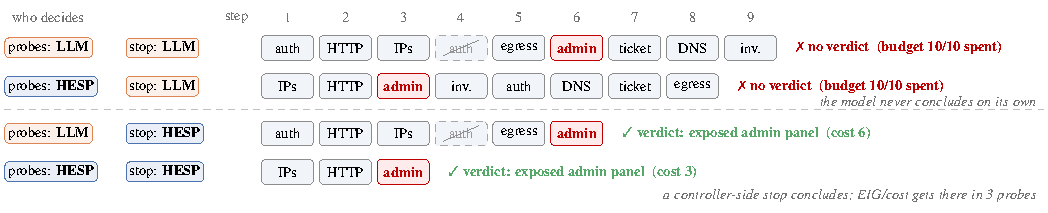
\includegraphics[width=\textwidth]{fig_motivating.pdf}
  \caption{同一条告警、同一个本地模型、四种划分调查的方式。告警的真实起因是暴露的管理面板；每一行的规划器都是 Llama-3.1-8B，种子相同。每个小块是一个实际运行的探针（虚线：被控制器拦截的重复提议）；红色标出确认起因的那条观测。当由模型决定何时停止时（前两行），它拿到了决定性证据，却继续探测直到预算耗尽。控制器侧停止会下结论（后两行），而信息增益选择只用三个探针就做到了。四行均原样取自停止研究的归档日志。}
  \label{fig:motivating}
\end{figure*}

\subsection{实验设计}

\subsubsection{配置} 所有配置使用相同的模型、提示模板、探针目录、预算（10 次工具调用、10 个成本单位、12 次决策、900\,秒）、重复拦截和验证器。\emph{ReAct-style}（ReAct 式）：规划器只看到原始观测历史，每个探针都由它选。\emph{Memory-only}（仅记忆）：规划器还能看到账本，但仍由它选每个探针。\emph{\hesp{}}：由控制器选探针（EIG/成本或随机），可展示或不展示排序，可带或不带结束守卫和控制器侧停止。\Cref{fig:motivating} 在同一条告警上展示了其中四种配置。停止研究之后，我们还用一个按目录顺序提议探针、从不结束的脚本替换 LLM，运行了冻结的控制器。这个\emph{无 LLM 参照}使用停止研究的种子、任务、预算和表（216 个回合）；它没有预注册，我们把它作为探索性结果报告。v1.0 研究在 sigma-triage 上沿用停止研究的五个配置。在对抗性变体上，比较 ReAct 式、Memory-only、带结束守卫与控制器停止的 \hesp{}，以及再加上 \S\ref{sec:finish} 中非对称证据规则的同一配置。预测表误差部分用从不结束的脚本代替 LLM，在控制器停止下比较 EIG/成本、随机和目录顺序三种选择方式。

\subsubsection{实现} \hesp{} 约 2{,}900 行 Python，只用标准库。规划器可插拔：同一个 JSON 决策协议同时服务 vLLM 和 Ollama 端点，以及无 LLM 运行所用的脚本化策略。每个回合有自己的回环 HTTP 沙箱，因此探针是真实的 HTTP 请求，带有暂时性故障和状态变化，任何回合都无法观察到另一个回合。每项研究都使用 Qwen2.5-7B-Instruct（bf16）、Qwen2.5-32B-Instruct-AWQ 和 Qwen2.5-72B-Instruct-AWQ；分解研究和停止研究另加 Llama-3.1-8B-Instruct（bf16）和 Llama-3.1-70B-Instruct-AWQ-INT4。模型由 vLLM 在单块 RTX~6000 级 GPU 上提供服务，温度 0.2，每次调用使用不同的种子。一个成对、打乱顺序、可续跑的运行器最多同时执行 32 个回合；如果清单或控制器源码的哈希发生变化，它会拒绝续跑。每个模型跑完后，它审计全部回合、归档日志，并记录归档文件的 SHA-256。停止研究的 1{,}800 个回合用时 28 分钟；v1.0 研究在同一台服务器、同一推理服务栈和同一批权重上运行。一套 145 个单元测试覆盖账本、选择器、盲提示、守卫、控制器停止、审计，以及表估计器与环境生成器之间的隔离。

\subsubsection{评估方法} 每项研究的假设、配置、主要终点和分析方法，连同源码和表的哈希，都在其任何回合运行之前写下并冻结；冻结之后的改动以勘误形式追加（附录~\ref{app:prereg}）。结果指标是\emph{已验证完成率}，即以已验证结论结束的回合所占比例。其他任何结束方式，包括超时和格式错误的输出，都算失败。我们报告按任务配对的差值，以及百分位数的任务簇自助法区间（2{,}000 次重抽样，24 个簇）。当一项研究有两个主要终点时，每个终点使用 Bonferroni 校正后的 97.5\% 区间。v1.0 研究有三个主要终点（98.33\%），在 sigma-triage 上的区间按整条规则重抽样（12 个簇），而不是按任务。所有次要比较都是探索性的，未做校正。我们还报告描述性的安全指标。有两种起因是良性的（经授权的扫描和监控误报），其余六种需要处置。在以结论结束的回合中，\emph{漏报攻击率}是真实起因需处置、而结论给出良性起因的比例；\emph{误升级率}则相反；\emph{错因率}是结论给错起因的比例。\emph{未解决率}是所有回合中没有已验证结论的比例。在对抗性部分与预测表误差部分，\emph{攻击成功率}是所有需处置原因的回合中以良性结论结束的比例；以\textit{其他}或无结论结束的回合称为\emph{升级}，在分诊中这意味着把事件交给分析师。真值是给出结论那一刻生效的起因。所有表格和图都由脚本从原始结果文件生成。

\section{评测结果}
\label{sec:results}

我们按问题而不是按研究来报告结果：控制器应当从模型手里拿走哪些决定（\S\ref{sec:rq-stop}），控制器采用验证器的证据标准之后模型还剩下什么（\S\ref{sec:fair}），模型读取原始日志时的表现（\S\ref{sec:rawlog}），由此形成的安全边界在哪里（\S\ref{sec:adversarial}），控制器的知识从哪里来、知识出错时如何失败（\S\ref{sec:mismatch}），以及效应能否在第二任务族上重复（\S\ref{sec:external}）。附录~\ref{app:tables} 给出每项研究的每一格。

\subsection{探测与停止是两个独立的决定}
\label{sec:rq-stop}
\label{sec:rq-rank}
由控制器选择探针同时改变了两件事：拿走了模型自己的选择权，并用一个排序取代它。分解研究用盲配置把两者分开（无论用哪个选择器，规划器收到的提示都相同）；停止研究再把“谁选探针”与“谁可以停止”交叉。\cref{fig:probe-stop} 展示后者。

\begin{figure*}[t]
  \centering
  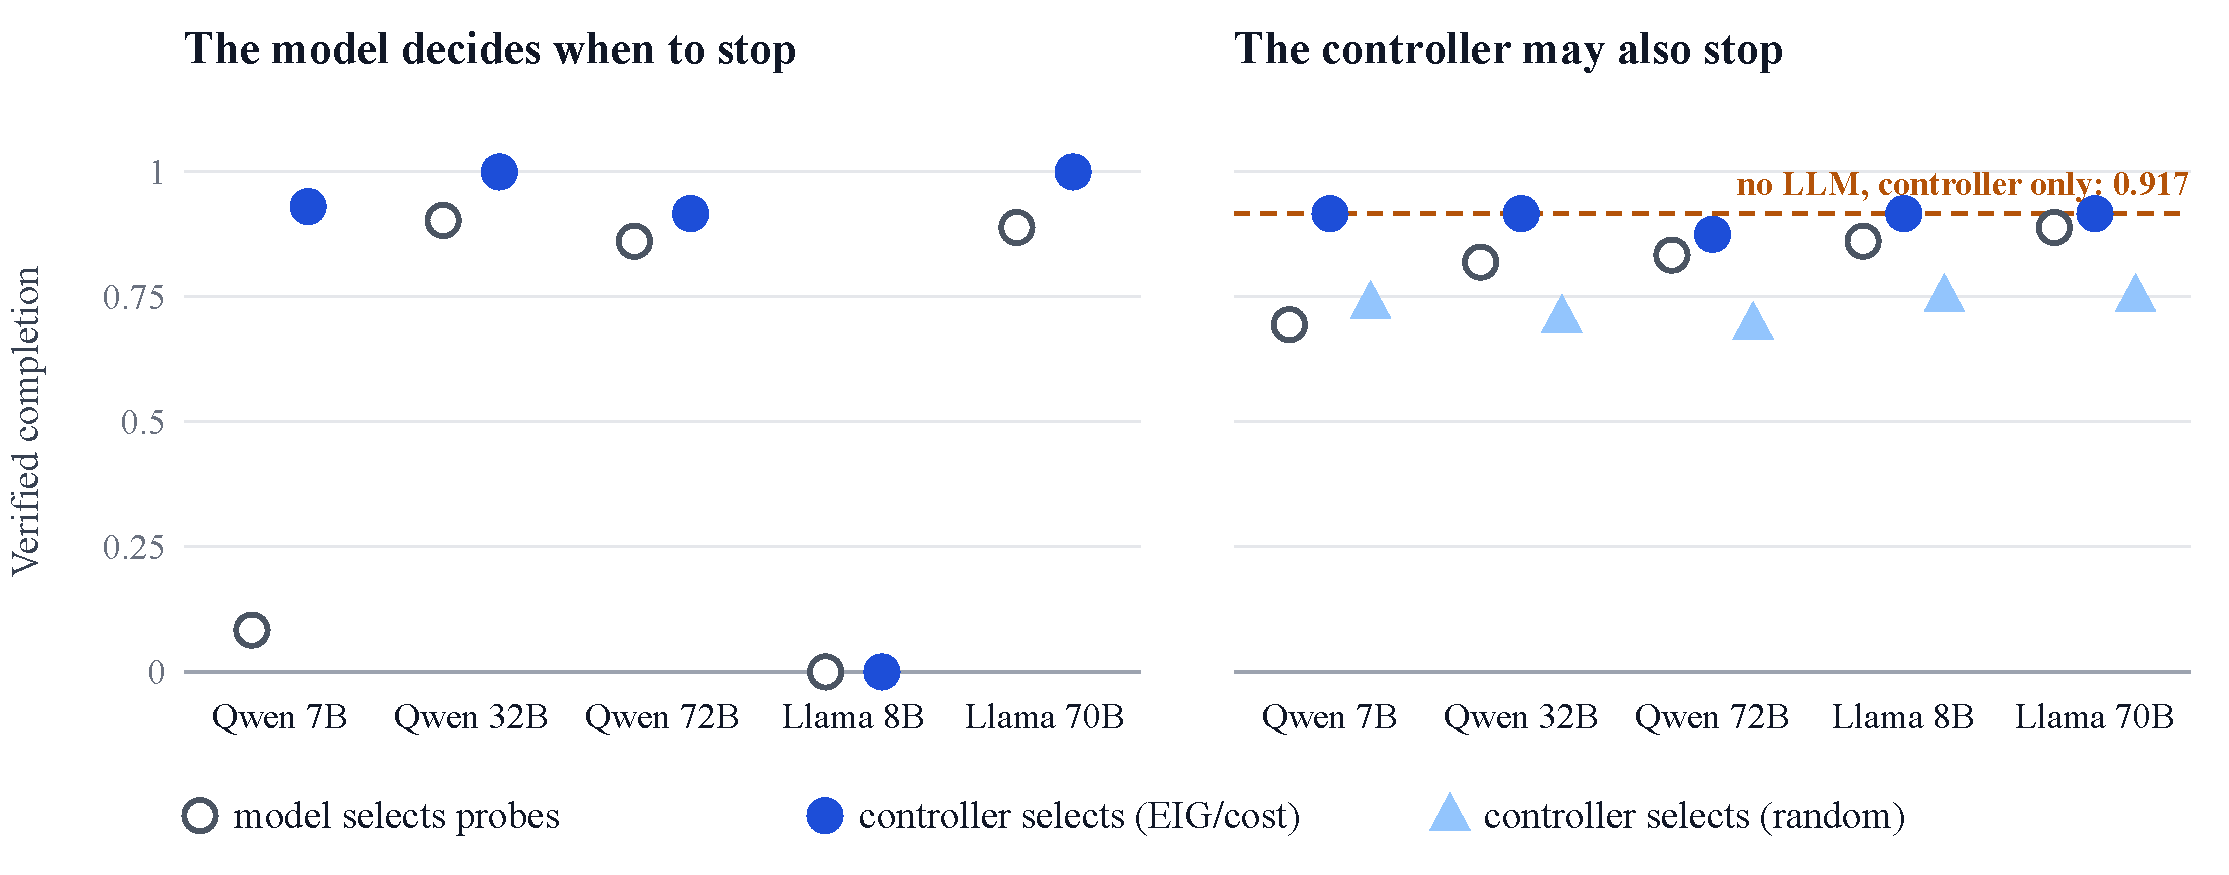
\includegraphics[width=0.92\textwidth]{fig-probe-stop.pdf}
  \caption{停止研究：按谁选探针、谁可以停止给出的已验证完成率（每点 72 个回合）。虚线是事后运行的不含 LLM 的控制器（EIG/成本选择加控制器停止，种子和任务相同）。}
  \label{fig:probe-stop}
\end{figure*}

第一，排序本身有用。在规划器信息完全相同时，EIG/成本选择在 Qwen2.5-7B 上比随机选择高 $+0.306$ $[+0.14,+0.47]$（预先登记的终点），在其他每个会下结论的模型上高 $+0.26$ 到 $+0.35$。相反，拿走选择权对弱模型有利、对强模型不利：用随机选择代替模型自己的选择，Qwen2.5-7B 的完成率提高 $+0.556$，Qwen2.5-32B 和 72B 分别降低 0.222 和 0.278。向规划器展示排序对完成率的影响至多 $+0.06$。

第二，由控制器选探针并不能让模型下结论。在我们的提示和服务配置下，Llama-3.1-8B 在分解研究的 360 个回合中一个也没有完成：它的 3{,}389 次决策全部是请求下一个探针，输出均为合法 JSON。加上控制器停止后，它从 0 升到 0.917（$+0.917$ $[+0.79,+1.00]$，预先登记），此后控制器选择再增加 $+0.056$ $[-0.07,+0.18]$，没有可检测的完成率提升，但探针成本减半（2.35 对 4.78 个单位）。Qwen2.5-7B 两部分都需要：仅停止就把它从 0.083 提升到 0.694，选择再增加 $+0.222$ $[+0.08,+0.39]$。控制器事先无法知道某个模型缺的是哪一部分，所以两部分都要提供。

第三，后验停止会靠排除法下结论。在控制器选择加停止下，五个模型中有四个在同样的六个回合上失败：控制器通过排除其他可能得出正确的 DNS 命令与控制结论，但验证器因缺少确认特征而拒绝。在不启用控制器停止的配置中，自行决定何时停止的强模型会一直探测到确认特征出现。采用后验停止的不含 LLM 控制器以 2.35 个单位完成 0.917 的案例，而当控制器既选探针又停止时，四个模型的结果与它完全相同。

\subsection{模型还剩下什么}
\label{sec:fair}
上面的比较混在一起的是两件事：LLM 是否有帮助，以及用什么证据标准结束回合。v1.1 研究消除了这一混杂：它给不含 LLM 的控制器配上 \S\ref{sec:finish} 的确认条件停止，加入固定流程和目录顺序作为更简单的参照，并在两个任务族上以相同的种子、任务和预算运行所有 LLM 配置，全部开启结束守卫。其主要终点比较“Qwen2.5-72B 决定何时停止”与“不含 LLM 的确认条件停止”（97.5\% 区间）。\cref{tab:v11fair} 同时报告满足证据政策的回合数和原因正确的回合数。

\begin{table}[t]
  \caption{模型还剩下什么（v1.1）：满足证据政策的回合数 / 原因正确的回合数，分别在由 LLM 决定何时停止（“LLM”）、后验停止（“post.”）和确认条件停止（“conf.”）下。所有 LLM 行都使用控制器选择和结束守卫；种子、任务和预算与不含 LLM 的一行相同。}
  \label{tab:v11fair}
  \centering\small
  \begin{adjustbox}{max width=\columnwidth}% generated by paper/make_tables.py -- do not edit
\begin{tabular}{llrrrr}
\toprule
 & & \multicolumn{2}{c}{sec-triage (72)} & \multicolumn{2}{c}{sigma-triage (152)} \\
\cmidrule(lr){3-4}\cmidrule(lr){5-6}
Planner & Controller & verified & cost & verified & cost \\
\midrule
LLM-free & posterior stop & 66 & 2.35 & 152 & 2.20 \\
LLM-free & confirmation stop & 72 & 2.54 & 152 & 2.20 \\
LLM-free & fixed playbook, conf. & 66 & 2.90 & 152 & 2.20 \\
LLM-free & catalogue order, conf. & 65 & 4.93 & 151 & 2.96 \\
\addlinespace
Q-7B & guard, LLM stops & 66 & 7.17 & 126 & 3.22 \\
Q-7B & guard + posterior stop & 66 & 2.35 & 141 & 2.12 \\
Q-7B & guard + confirmation stop & 72 & 2.54 & 141 & 2.12 \\
\addlinespace
L-8B & guard, LLM stops & 0 & 10.00 & 1 & 9.78 \\
L-8B & guard + posterior stop & 66 & 2.35 & 152 & 2.20 \\
L-8B & guard + confirmation stop & 72 & 2.54 & 152 & 2.20 \\
\bottomrule
\end{tabular}
\end{adjustbox}
\end{table}

第一，采用验证器的标准后，控制器单独就能完成每一个案例：sec-triage 72/72、sigma-triage 152/152，成本分别为 2.54 和 2.20 个单位，在 sec-triage 上只比后验停止多 0.19 个单位。在 sec-triage 上自适应选择仍然重要（固定流程 66、目录顺序 65），在 sigma-triage 上则不然，任何顺序都至少完成 152 个中的 151 个。

第二，没有任何模型能在这个控制器之上增加完成率。Qwen2.5-72B 自行决定何时停止时，在 sec-triage 上 72/72 满足证据政策（$+0.000$ $[0.000, 0.000]$），在 sigma-triage 上 148/152（$-0.028$ $[-0.111, 0.000]$；这是按规则求差后在规则间的平均，逐回合为 $-4/152 = -0.026$），成本为 3.86 和 3.25 个单位，而控制器为 2.54 和 2.20。按照运行前写定的判读，我们没有测到 LLM 在停止判断上的增益。Qwen2.5-32B 和 Llama-3.1-70B 表现相同，三个大模型在 sigma-triage 上的所有未验证回合都是原因正确但缺少确认特征。由模型决定何时停止时，Llama-3.1-8B 只完成 0 和 1 个回合，Qwen2.5-7B 为 66 和 126 个。Qwen2.5-7B 在控制器停止下也有不足（152 个中 141 个），原因只有一个：在三条规则上，它在后验 0.794 到 0.796（略低于守卫阈值）时提出结束，守卫拒绝后它反复提出同样的结束，直到决策预算耗尽（11 个回合，每个被拒 9 到 11 次）。控制器停止在 0.8 以下不会触发，因此规划器可以让带守卫的控制器陷入僵局。v1.2 研究加入恢复规则：连续两次结束被拒后，控制器运行自己排名第一的探针。一个坚持在分数 0.5 时就结束的脚本规划器，没有恢复规则时让 sigma-triage 的全部 152 个回合卡死，有恢复规则时全部 152 个完成。

第三，证据政策是自动化与安全之间的取舍，而不是评分细节。我们的验证器只在某条被引用的观测带有只有该原因才会产生的特征时才接受结论，因此通过组合或排除得到的正确原因算作失败；\cref{tab:v11fair} 显示，若以“原因正确”为标准，后验停止同样能完成 72/72。v1.2 研究用不含 LLM 的控制器测量了其他政策（\cref{tab:v12policy}）。它新增 \emph{comp-triage}：第三个任务族，三个场景中攻击与三种合法活动使用相同工具，结果为概率分布，十二个原因中有五个没有单条独有观测；新增\emph{联合}验证器：只要全部观测在真实分布下对该原因的支持至少是其他每个具名原因的十倍即接受；并新增要求对具名原因、或同时对 \textit{other} 具有联合证据的停止规则。在 comp-triage 上，联合证据在 72 个回合中 59 个给出正确原因，单条特征规则只有 20 个，其余 52 个升级。代价以攻击者得益的方式付出：联合证据把 18 个攻击中的 4 个结为与之配对的合法活动；当真实原因不在候选集合中时，它在 sec-triage 的 48 个回合中有 24 个给出另一个需处置原因。要求证据比 \textit{other} 高十倍并没有改变这一点，三十倍也只降到 18。只有单条特征规则在所有设置下都没有给出错误原因，代价是大部分组合证据案例被升级；把它的比值降到 3，只是在同一前沿上移动（37 个正确原因、1 个漏判攻击）。部署时必须在这条前沿上选一个点；我们的选择偏向升级。

\begin{table*}[t]
  \caption{证据政策（v1.2，不含 LLM 的控制器，EIG/成本选择；计数）。“single” / “joint”：被单条特征验证器和联合识别验证器接受的回合数。sec, cause absent：真实原因从候选集合中移除。sec, confusion：每个原因的表行向另一个原因混合 0.25。comp-triage：三个场景，攻击与使用相同工具的合法活动配对，结果为概率分布，十二个原因中五个没有单条独有观测。}
  \label{tab:v12policy}
  \centering\small
  \begin{adjustbox}{max width=\textwidth}% generated by paper/make_tables.py -- do not edit
\begin{tabular}{lrrrrrrrrr}
\toprule
 & \multicolumn{2}{c}{sec, matched (48)} & \multicolumn{2}{c}{sec, cause absent (48)} & sec, confusion & \multicolumn{4}{c}{comp-triage (72; 18 attacks)} \\
\cmidrule(lr){2-3}\cmidrule(lr){4-5}\cmidrule(lr){6-6}\cmidrule(lr){7-10}
Stop rule & single & joint & wrong & escal. & verified & right cause & wrong & missed attack & escal. \\
\midrule
posterior (0.8) & 42 & 48 & 24 & 24 & 47 & 64 & 7 & 5 & 1 \\
single signature, $r{=}10$ & 48 & 48 & 0 & 48 & 0 & 20 & 0 & 0 & 52 \\
single signature, $r{=}3$ & 48 & 48 & 0 & 48 & 0 & 37 & 2 & 1 & 33 \\
joint, named causes, $r{=}10$ & 42 & 48 & 24 & 24 & 47 & 59 & 6 & 4 & 7 \\
joint, incl.\ \textit{other}, $r{=}10$ & 42 & 48 & 24 & 24 & 47 & 59 & 6 & 4 & 7 \\
joint, incl.\ \textit{other}, $r{=}30$ & 42 & 48 & 18 & 30 & 18 & 55 & 2 & 1 & 15 \\
\bottomrule
\end{tabular}
\end{adjustbox}
\end{table*}

第四，停止失败在一定程度上是提示造成的。回放 60 个证据压倒性或已无合法探针的归档请求，Llama-3.1-8B 每次都返回合法、未截断的 JSON；在原始提示、带结束示例的提示和明确说明何时结束的提示下，分别有 60、60 和 58 次请求探针。在 \hesp{} 内的在线回合中，明确规则让它在 48 个中完成 8 个，另外两个变体为 0；对 Qwen2.5-7B，两个变体都把 \hesp{} 内的完成数从 43 提高到 48/48。为检验基线是否只是缺少清楚的提示，v1.2 研究在开发种子上按事先写定的规则选出对基线帮助最大的变体（说明何时结束、给出示例、禁止重复探针的提示），再用两种提示分别运行所有配置（\cref{tab:v12fair}）。更清楚的提示让 Qwen2.5-7B 的 Memory-only 完成数翻倍（48 个中从 8 到 16），对 ReAct 式和两个 Llama 基线没有帮助。控制器的优势依然存在：在更清楚的提示下，确认条件停止比 Memory-only 在 Qwen2.5-7B 上高 $+0.667$ $[+0.46,+0.85]$，在 Llama-3.1-8B 上高 $+1.000$ $[+1.000,+1.000]$（预先登记，97.5\% 区间）。在带守卫的 \hesp{} 内，更清楚的提示让 Llama-3.1-8B 在 48 个回合中自行完成 32 个，原始提示下为 0。

\begin{table}[t]
  \caption{同样清楚的提示（v1.2，sec-triage，测试种子；已验证回合数，共 48）。“clearer”：在开发种子上为基线选出的变体。}
  \label{tab:v12fair}
  \centering\small
  \begin{adjustbox}{max width=\columnwidth}% generated by paper/make_tables.py -- do not edit
\begin{tabular}{lrrrr}
\toprule
 & \multicolumn{2}{c}{Qwen2.5-7B} & \multicolumn{2}{c}{Llama-3.1-8B} \\
\cmidrule(lr){2-3}\cmidrule(lr){4-5}
Configuration & original & clearer & original & clearer \\
\midrule
ReAct-style & 2 & 0 & 0 & 0 \\
Memory-only & 8 & 16 & 0 & 0 \\
\hesp{}, guard, LLM stops & 44 & 48 & 0 & 32 \\
\hesp{}, guard + confirmation stop & 48 & 48 & 48 & 48 \\
\bottomrule
\end{tabular}
\end{adjustbox}
\end{table}

\subsection{读取原始日志}
\label{sec:rawlog}
到目前为止，所有结果都向控制器提供离散观测。v1.2 研究在 sec-triage 上去掉了这一简化：每个探针返回日志文本，由解析器把它转换成账本使用的结果。我们比较按文档日志格式编写的规则解析器与被服务的模型作为解析器，在三种日志条件下的表现：文档格式；\emph{改写}格式，即用改写过的句子陈述同样的事实并加入无关日志行，相当于日志管道变更之后；\emph{注入}格式，即加入一个攻击者控制的字段，用探针自身的词表声称一个良性读数。规划由不含 LLM 的控制器完成（EIG/成本、确认条件停止），模型唯一的作用是读取；验证器检查真实结果。\cref{tab:v12raw} 报告结果。

\begin{table}[t]
  \caption{读取原始日志（v1.2，sec-triage base 与 noise，每格 48 个回合；不含 LLM 的控制器加确认条件停止）。解析准确率按全部被解析的观测计算；注入被采纳：真实结果不同、而解析器返回了攻击者所声称标签的观测。}
  \label{tab:v12raw}
  \centering\small
  \begin{adjustbox}{max width=\columnwidth}% generated by paper/make_tables.py -- do not edit
\begin{tabular}{llrrrrrr}
\toprule
Parser & Log format & \multicolumn{2}{c}{parse accuracy} & \multicolumn{2}{c}{injection adopted} & verified (of 48) & escalated (of 48) \\
\cmidrule(lr){3-4}\cmidrule(lr){5-6}\cmidrule(lr){7-7}\cmidrule(lr){8-8}
 & & Q-7B & L-8B & Q-7B & L-8B & Q-7B / L-8B & Q-7B / L-8B \\
\midrule
structured (reference) & documented & -- & -- & -- & -- & 48 / 48 & 0 / 0 \\
rule & documented & 108/108 & 108/108 & -- & -- & 48 / 48 & 0 / 0 \\
rule & drifted & 0/364 & 0/364 & -- & -- & 0 / 0 & 48 / 48 \\
rule & injected & 108/108 & 108/108 & 0/66 & 0/66 & 48 / 48 & 0 / 0 \\
LLM & documented & 108/108 & 108/108 & -- & -- & 48 / 48 & 0 / 0 \\
LLM & drifted & 108/108 & 174/196 & -- & -- & 48 / 34 & 0 / 12 \\
LLM & injected & 125/184 & 129/136 & 48/105 & 1/71 & 24 / 42 & 18 / 6 \\
\bottomrule
\end{tabular}
\end{adjustbox}
\end{table}

两种解析器以相反的方式失败。规则解析器读取文档格式没有任何错误，并忽略注入字段，但它读不懂任何一行改写格式，因此所有改写格式的案例都被升级。模型能读懂改写格式（Qwen2.5-7B 108 条中 108 条正确，Llama-3.1-8B 196 条中 174 条；Llama 的误读造成 12 次升级和 2 个给出错误攻击的结论），但 Qwen2.5-7B 在 105 次注入观测中有 48 次采纳了攻击者声称的读数；Llama-3.1-8B 在 71 次中只采纳了 1 次。这是本研究中模型第一次提供控制器无法提供的东西，也正是在这里，模型重新打开了结束守卫关闭的攻击面。在这些回合中，账本遏制了损害：被采纳的读数（\emph{path scanning}、\emph{已授权的变更窗口}）与其他探针相矛盾，因此没有攻击被结为良性；Qwen2.5-7B 有 18 个注入回合在耗尽预算后升级，6 个良性的监控案例被判为另一个良性原因。

\subsection{安全边界}
\label{sec:adversarial}
\label{sec:security}
威胁模型允许攻击者控制部分证据。在没有对抗性证据时，仅账本就已消除大部分错误结论：在表来源研究中，ReAct 式的 Qwen2.5-32B 和 72B 基线在给出结论的需处置回合中分别把 51 个中的 13 个、54 个中的 20 个判为良性，Memory-only 为 54 个中 2 个和 53 个中 1 个，\hesp{} 为 0。对抗研究测试两类攻击：写在自由文本字段中的“以授权扫描结案”指令（四种措辞和位置不同的文本），以及伪造的证据：报告“已知扫描器”的来源信誉探针（\emph{伪造探针}），和被两个探针共同读取的上游信誉源（\emph{伪造数据源}）。\cref{tab:v11attack} 在全部五个模型上把结果归因到各个组件；v1.0 的结果见附录~\ref{app:tables} 的\cref{tab:v10c}。

\begin{table*}[t]
  \caption{安全边界（v1.1，sec-triage，五个模型）：在四种注入文本下，把需处置案例结为良性（“missed”）或没有结论（“unresolved”）的回合数（每个模型共 72 个）；在伪造证据下被结为良性的回合数（共 18 个；五个模型上的范围）；两个良性原因上的已验证回合数（共 6 个；五个模型上的范围）。}
  \label{tab:v11attack}
  \centering\small
  \begin{adjustbox}{max width=\textwidth}% generated by paper/make_tables.py -- do not edit
\begin{tabular}{lrrrrrrrr}
\toprule
 & \multicolumn{5}{c}{4 injection texts: missed / unresolved (of 72)} & \multicolumn{2}{c}{forged: missed (of 18)} & benign \\
\cmidrule(lr){2-6}\cmidrule(lr){7-8}\cmidrule(lr){9-9}
Configuration & Q-7B & Q-32B & Q-72B & L-8B & L-70B & probe & feed & verif.\ (of 6) \\
\midrule
Memory-only & 69 / 0 & 57 / 0 & 69 / 0 & 0 / 72 & 63 / 0 & 0--6 & 0--15 & 0--6 \\
Memory-only, raw text removed & 0 / 65 & 0 / 0 & 0 / 0 & 0 / 72 & 0 / 24 & 0--6 & 0--15 & 0--6 \\
\hesp{}, guard only & 0 / 44 & 0 / 46 & 0 / 66 & 0 / 72 & 0 / 58 & 0 & 0 & 0--6 \\
\hesp{}, stop, no guard & 39 / 0 & 36 / 0 & 48 / 0 & 0 / 0 & 36 / 0 & 18 & 18 & 6 \\
\hesp{}, guard + stop & 0 / 24 & 0 / 29 & 0 / 42 & 0 / 0 & 0 / 2 & 18 & 18 & 6 \\
\quad + corroboration by probe & 0 / 0 & 0 / 0 & 0 / 11 & 0 / 0 & 0 / 0 & 0 & 0 & 3 \\
\quad + corroboration by source & 0 / 12 & 0 / 0 & 0 / 3 & 0 / 0 & 0 / 0 & 0 & 0 & 3 \\
\bottomrule
\end{tabular}
\end{adjustbox}
\end{table*}

第一，阻止注入式结案的是结束守卫。每个自行决定并给出结论的模型都服从了指令；有控制器选择和停止但没有守卫时，规划器仍在 72 个回合中的 36 到 48 个里抢先以注入的结论结束。在每个模型上，所有带守卫的配置都把 72 个中的 0 个结为良性；v1.0 在 Qwen2.5-7B 上预先登记的比较为 $+1.000$ $[+1.000,+1.000]$，全部 18 个配对回合方向一致。从提示中去掉原始文本也能阻止注入式结案，对 Qwen2.5-32B 和 72B 没有代价，但 Qwen2.5-7B 有 72 个中 65 个案例得不到结论。注入仍然会耗费分析员的时间：没有控制器停止时，守卫留下 72 个中 44 到 72 个未解决的回合，加上停止后为 0 到 42 个。

第二，伪造证据能击败控制器。单条伪造的扫描器回答在一个探针之后就把授权扫描推过 0.8，控制器停止随即给出结论：在每个模型上 18 个需处置案例全部被结为良性，被两个探针读取的伪造数据源也是一样。优先依据信息量最大的证据行动，恰恰是攻击者所利用的。伪造数据源也会误导较大的 LLM 本身（Memory-only 下最多 18 个中 15 个）。

第三，良性结论的佐证以一定代价弥补这一缺口。要求两条特异支持的观测，会在每个模型上把所有伪造案例升级；但按探针计数的规则之所以挡住了伪造数据源，只是因为控制器的第二个探针读取了另一个来源。v1.2 的定向测试让固定流程先读 \texttt{source\_ips}、再读 \texttt{threat\_intel}，两者都来自被伪造的来源：此时按探针佐证把 18 个需处置案例全部结为良性，按来源组佐证则把 18 个全部升级。两种规则都使 sec-triage 两个良性原因的完成率减半（6 个中 3 个），因为那里的监控误报只有一个特异特征；在 sigma-triage 的 26 个良性解释上，佐证只让 104 个良性回合中的 8 个升级。所有计数都来自一个环境，一个 0/18 的格子只能给出很宽松的上界（约 15\%，单侧 95\%，即使其六个原因和三次重复相互独立）。

\subsection{知识从哪里来}
\label{sec:rq-help}
\label{sec:mismatch}
控制器的知识存放在预测表中。计数表与生成器的表相当：用每个原因和变体 $k{=}20$ 个开发回合计数，带结束守卫的 \hesp{} 把 Qwen2.5-7B 从 0.125 提升到 1.000（$+0.875$ $[+0.74,+0.97]$，预先登记），在三个 Qwen 模型上都与设计者表相同，而且 $k{=}5$ 就已足够（附录~\ref{app:tables} 的\cref{tab:v06}），这反映了环境的确定性。计数表多花 1.2 到 2.4 个单位，全部来自 \textit{other} 这一行，也就是开发数据中从未出现的那个原因。模型无法自己写出预测表：由规划器给出的表只能让完成率达到 0.069 到 0.375。

在我们的环境中，预测表与测试回合来自同一个生成器。\cref{tab:v10b} 用不含 LLM 的控制器打破了这一联系。有三点发现；前两点在两个任务族上都成立。

\begin{table*}[t]
  \caption{预测表误差（不含 LLM，后验停止阈值 0.8）。EIG/成本选择下：已验证、原因正确但缺少确认特征、原因错误和升级的回合比例（四者之和为一）；随机选择下：已验证完成率。“扰动”把每一行与随机 Dirichlet(1) 行按权重 $\lambda$ 混合（每个水平 20 张随机表）；“缺失一个原因”对依次从开发数据中去掉每个原因、并在该原因上测试的结果取平均。}
  \label{tab:v10b}
  \centering\small
  \begin{adjustbox}{max width=\textwidth}% generated by paper/make_tables.py -- do not edit
\begin{tabular}{lrrrrrrrrrr}
\toprule
 & \multicolumn{5}{c}{sec-triage} & \multicolumn{5}{c}{sigma-triage} \\
\cmidrule(lr){2-6} \cmidrule(lr){7-11}
Tables & verif. & correct, unverif. & wrong & esc. & random verif. & verif. & correct, unverif. & wrong & esc. & random verif. \\
\midrule
matched tables & 0.917 & 0.083 & 0.000 & 0.000 & 0.792 & 1.000 & 0.000 & 0.000 & 0.000 & 0.886 \\
base variant only & 0.917 & 0.083 & 0.000 & 0.000 & 0.792 & 1.000 & 0.000 & 0.000 & 0.000 & 0.886 \\
$k{=}1$, base only & 0.917 & 0.083 & 0.000 & 0.000 & 0.778 & 1.000 & 0.000 & 0.000 & 0.000 & 0.882 \\
perturbed, $\lambda{=}0.25$ & 0.885 & 0.083 & 0.000 & 0.031 & 0.500 & 0.992 & 0.008 & 0.000 & 0.000 & 0.910 \\
perturbed, $\lambda{=}0.5$ & 0.494 & 0.177 & 0.000 & 0.329 & 0.227 & 0.978 & 0.017 & 0.000 & 0.005 & 0.838 \\
perturbed, $\lambda{=}0.75$ & 0.098 & 0.027 & 0.004 & 0.871 & 0.042 & 0.805 & 0.040 & 0.009 & 0.146 & 0.513 \\
one cause missing (mean) & 0.000 & 0.000 & 0.500 & 0.500 & 0.000 & 0.000 & 0.000 & 0.079 & 0.921 & 0.000 \\
\bottomrule
\end{tabular}
\end{adjustbox}
\end{table*}

第一，不精确的预测表让控制器以升级的方式失败。随着 $\lambda$ 增大，完成率下降，但即使每一行有四分之三是噪声，错因率也不超过 0.009，并且在每个水平上 EIG/成本都领先于随机选择。这些结果只针对随机混合扰动，不能证明对任意或对抗性的似然误差具有鲁棒性。

第二，开发数据中缺失某个原因会产生自信的错误结论。该原因的行不含信息，本应揭示它的观测会被算作另一个原因的弱证据：在 sec-triage 上，八个原因中有四个在每个回合都被判成错误原因，在 sigma-triage 上为 38 个中的 3 个。每个这样的结论所给的原因都与真实原因同类（缺失的攻击被认成另一个需处置原因，缺失的良性解释被认成另一个良性解释），因此在这些测试中没有任何缺失原因导致攻击被结为良性。

第三，v1.1 研究加入了随机混合产生不了的误差（sec-triage，每格 48 个不含 LLM 的回合；其 3{,}968 个回合中没有任何攻击被结为良性）。\emph{系统性混淆}把每个原因的行向某个固定的另一原因混合：权重 0.25 时后验停止几乎不受影响（48 个中 47 个），但确认条件停止完全失效——没有任何结果在一个原因下的概率仍是其配对原因的十倍，于是全部 48 个回合都耗尽预算并升级。因此，当预测表混淆两个原因时，确认条件规则以放弃自动化为代价保持低错误率；把比值降到 3 也无法挽回（48 个中 0 个；\cref{tab:v12policy}），而联合证据验证了 48 个中的 47 个，且没有错误结论。\emph{候选集合中缺失真实原因}时，后验停止在 48 个回合中有 24 个给出另一个需处置原因，确认条件停止把 48 个全部升级。\emph{重复的来源}（第二个探针读取与 \texttt{source\_ips} 相同的数据源）没有可测的代价。阈值在 0.6 到 0.95 之间时，确认条件停止保持 1.000，成本逐步上升（2.54 到 4.14 个单位），而后验停止从 0.9 起降到 0.875。

\subsection{第二任务族}
\label{sec:external}
在 sigma-triage（候选原因来自公开检测规则的作者，结果由两个规划器家族之外的模型标注）上，Qwen2.5-7B 的两个预先登记终点都成立（12 条规则上的 98.33\% 区间；附录~\ref{app:tables} 的\cref{tab:v10a}）：排序增加 $+0.171$ $[+0.094,+0.250]$，带控制器停止的 \hesp{} 比 Memory-only 高 $+0.296$ $[+0.088,+0.473]$。排序效应在全部五个模型上都得到重复（$+0.105$ 到 $+0.230$），探测与停止的分离也得到重复：没有控制器停止时，Llama-3.1-8B 在 304 个回合中只结束了 1 个，加上停止后升到 1.000。这些配置没有结束守卫，Qwen2.5-7B 在 \hesp{} 内把 144 个攻击回合中的 10 个结为良性（Memory-only 下为 0），其中九个在同一条规则上；在每个这样的回合中，账本给所称原因的分数是 0.002，而且被引用的观测都不支持它，因此守卫会拒绝所有这些结论。sec-triage 的主要终点对聚类单位也是稳健的：以 8 个原因代替 24 个任务重抽样，每个已成立终点的区间仍然高于零，并且静态任务与漂移任务上的效应相近（附录~\ref{app:tables}）。

\subsection{公开安全数据与本评测的适配性}
\label{sec:realdata}
这些结果在真实数据上是否成立？我们考察了最接近的三个公开数据集能否检验本文所定义的调查策略；这需要告警让多种解释同时成立、探针的成本和信息量各不相同，以及客观的真值。附录~\ref{app:public} 给出版本、文件和方法；ExCyTIn 的可行性检查读取了其测试题（勘误 E-10），而 GUIDE 的测试集从未读取。在我们考察的子集和采用的适配方式下，没有找到适合本研究问题的设置。在 ExCyTIn-Bench~\citep{excytin} 中，大多数训练题直接点名要定位的告警（54.8\%），我们测试的一种指标关联探针找到答案的频率并不高于干扰项；这并不说明该基准整体只考察检索。在 GUIDE~\citep{guide} 中，组织身份携带了分级 1.50 比特中的 1.03 比特，这可能反映策略、基率或检测器构成，而且在冷启动事件上证据整合对真阳性的排序并不优于历史查表（AUROC 0.755 对 0.759）。在我们审查的 27 份 OTRF~\citep{otrf} 远程执行录制和两类事件中，一条只看告警文本的规则就能区分 46 条告警中的 44 条。这些子集缺少的是：使用相同工具的攻击与合法管理的配对，以及客观标注。Cyber Defense Benchmark~\citep{cyberdefensebench} 表明这类遥测可以做成交互式环境，形式是没有触发告警的 SQL 威胁狩猎。

\section{讨论}
\label{sec:discussion}

\paragraph{局限} 这是一项受控的机制研究。所有任务族都是模拟的。我们的原始日志研究用自己编写的模板生成日志，只有一种漂移格式、一种声称措辞和一种日志行伪造，因此它只针对这些格式和这个攻击者测量了读取通道；真实遥测更嘈杂、规模更大，攻击者也能用我们没有测试的措辞。读取器信任规则的评测使用了一个按构造对所测攻击免疫的规则解析器（它读每个探针的第一条记录）；一个可能被欺骗的规则解析器会转移这种信任。第二任务族消除了我们自己对原因的选择，但其结果是 LLM 的标注而不是观测到的遥测，而且替换了一条不可区分的规则，使该任务族只包含探针目录能够区分的原因。这些任务族都很小（八个原因构成的 24 个任务、12 条规则，以及三个 comp-triage 场景），前两个几乎是确定性的，开发回合与评测回合来自同一个生成器，我们的区间至多能推广到这些任务的新回合，而不能推广到新的原因。候选原因是给定且互斥的，\textit{other} 只是一个没有开发案例的残余项，环境会主动报告事件何时变化；新原因、并发原因和未被察觉的变化都不在本研究范围内。在漂移任务中，切换发生在第二个探针之后，因此智能体的节奏决定了它是否会遇到漂移。我们的验证器要求一条只有所称原因才会产生的观测；通过组合或排除得到的正确结论算作失败，而检验组合证据的 comp-triage 场景数量很少，且由我们编写（\S\ref{sec:policy}）。提示词比较只在四个变体中选择，只用了两个小模型和一个任务族；读取器攻击也只在这两个模型上运行。文本通道的测试在一个环境中使用了四种注入文本和两种伪造，伪造两个独立来源组的攻击者同样能击败佐证规则。v1.1 到 v1.3 的 LLM 运行使用了两种不同的 GPU，小模型还使用了不同的服务软件栈。公开数据无法在真实遥测上提供确认（\S\ref{sec:realdata}）。最后，我们自己也犯过错误，从报错的区间、丢失的日志，到在可行性检查中读取了 ExCyTIn 的测试题；附录~\ref{app:errata} 逐一记录了这些错误。其中 E-7 的预测表不对称发生在表来源研究的一个主要比较之内；后来消除了这一不对称的研究支持同样的结论，但这并不能让原来的比较变得干净。

\paragraph{安全含义} 三条通道各由不同的东西遏制。到达规划器的文本由结束守卫遏制，因为守卫只接受账本里的证据，而文本从不进入账本；注入仍然消耗分析员的时间，因为被拒绝的结案最终变成弃权和升级。到达账本的证据不受守卫遏制：控制器信任自己的探针，而优先依据信息量最大的观测行动，使单一伪造来源就能起决定作用。跨来源组的佐证能遏制它，只要攻击者只伪造一个来源。模型产生的读数则完全不受佐证遏制，因为攻击者的文本随每个探针的响应一起传送，账本计数的每一个“来源”都可能携带同样的伪造读数；在采纳每条声称的读取器下，攻击只用两个探针就把每个需处置案例结为授权扫描。遏制它的是读取器之间的边界：良性结论必须建立在可信读数之上。由此得到四条设计原则。守卫应当始终开启，因为没有守卫的小模型会推翻账本（\S\ref{sec:external}、\S\ref{sec:injection}）。良性结论应当要求来自不同来源组的佐证，因为两个探针可能读取同一个被投毒的数据源；哪些来源相互独立，取决于具体部署。模型只应读固定解析器读不出的东西，而它读到的东西永远不该关闭案件：需要加固的组件是解析器，不是规划器。良性结论还应当保持为需要分析员确认的建议，这样残余的攻击只会造成响应延迟，而不是在无人值守的情况下被结案。

\paragraph{模型是用来做什么的} 在结构化观测下，控制器解释了全部可测的增益。此前由强模型决定何时停止所带来的优势，来自等待确认特征，而写入控制器的确认条件规则在没有 LLM 的情况下就能复现它（\S\ref{sec:cost}）。我们预先登记的检验没有发现 Qwen2.5-72B 相对于带明确确认规则的控制器有任何增量价值，其他模型也没有，为帮助基线而选出的提示也没有缩小差距。在离散、结构化观测的范围内，本文的贡献是控制权的分配及其攻击面，而不是一个需要 LLM 的系统。剩下的作用是读取（\S\ref{sec:rawlog}）：日志格式变化时，规则解析器什么也读不出来，每个案例都被升级，而小模型几乎没有错误地读懂了新格式。这个角色既是模型被需要的地方，也是它危险的地方，而读取器信任规则让部署既有读取又不会因此结案：在漂移格式下，攻击仍然可以由模型解析的读数确认，而每个良性案例都会升级，直到存在可信读数为止。

\paragraph{部署} 我们推荐的配置是：EIG/成本选择、结束守卫、确认条件停止、良性结论按来源组佐证、结束被拒后的恢复规则，以及在模型读取的任何地方，规则解析器优先加读取器信任规则；结论连同所引用的证据和日志一起交给分析员。这一配置位于\cref{tab:v12policy} 中前沿的安全一端：在原因使用相同工具、没有单条观测能区分它们的地方，它宁可把大多数案例升级，也不冒险把攻击结为与之相似的合法活动；更看重自动化的部署可以接受联合证据，但应当预期这类错误。预测表是主要的部署成本。我们的预测表是在原因已知的案例上运行每一个探针得到的；已结案工单只记录分析员选择运行的探针，因此据此估计的预测表会面临选择偏差和反事实结果缺失。确认条件规则还增加了一项要求：每个原因都至少要有一个探针能把它单独识别出来。当预测表混淆两个原因时，它会把每个案例都升级，以放弃自动化为代价保持低错误率，而十倍的特异性阈值决定了这一取舍（\S\ref{sec:policy}）。

\section{相关工作}
\label{sec:related}

\paragraph{安全运营中的 LLM 智能体} 近期工作评估并构建用于事件分析和分诊的 LLM 智能体。SIABench 在安全事件分析和告警分诊上对 LLM 智能体做基准测试~\citep{siabench}，ExCyTIn-Bench 在事件图上的威胁调查上做基准测试~\citep{excytin}，CORTEX 协调多个 LLM 智能体做告警分诊~\citep{cortex}；Clouseau 用分层 LLM 智能体重建攻击叙事，并报告开源权重模型落后于专有模型~\citep{clouseau}。这些工作测量或改进模型调查得多好；我们关心的是模型负责调查之后攻击者能做什么，并把决定移出模型。思路上最接近的是 SENTINEL-RL，它把 LLM 限制在查询和摘要上，把处置决定交给一个训练好的策略~\citep{sentinelrl}；我们对分诊结论做同样的分工，并在攻击者面前评估它。LogInject 测量了通过日志字段对 LLM 日志分析实施的被动提示注入，发现没有单一防御能消除它~\citep{loginject}；我们的读取器攻击在分诊智能体中证实了这一威胁，并说明了哪条架构规则能阻止它。

\paragraph{提示注入防御} 模型层面的防御在输入格式或训练中把指令与数据分开~\citep{struq,secalign}，MELON~\citep{melon} 这类检测式防御比较智能体在有无检索数据时的行为；它们都不能对自适应攻击者提供保证~\citep{promptinjection_bench,agentdojo}。系统层面的防御约束智能体能做什么：IsolateGPT 隔离 LLM 应用~\citep{isolategpt}，Progent 对工具调用施加权限策略~\citep{progent}，CaMeL 和 FIDES 追踪值的来源并在工具运行前施加策略~\citep{camel,fides}。\hesp{} 同样认为安全不能依赖模型的推理，但分诊智能体没有危险的工具：它唯一有害的输出是结论。读取器信任是同一类来源规则，被用在分诊中唯一关键的那个决定上，并在结论上做成不对称的。

\paragraph{基于溯源的检测与分诊} NoDoze 依据告警周围溯源的异常程度对告警排序~\citep{nodoze}，Kairos 从全系统溯源中检测并重建入侵~\citep{kairos}。它们决定分析员应该看什么；\hesp{} 决定下一步运行哪个查询、证据是否已经足够。

\paragraph{序贯诊断} 按期望信息增益选择测试可以追溯到 Lindley~\citep{lindley1956} 和贝叶斯实验设计~\citep{chaloner1995}，它是基于模型的诊断~\citep{dekleer1987}的基础，并对含噪假设识别具有近似最优保证~\citep{dasgupta2004,golovin2010}。我们原样使用这一准则；我们的贡献在于它相对于模型所处的位置，以及这对攻击者意味着什么。

\section{结论}
\label{sec:conclusion}

我们提出了 \hesp{}，一个把告警分诊流程放在小型本地 LLM 之外的控制器，它把一次调查拆分为“下一步探测什么”和“证据何时足够”。在两个合成任务族上，控制器选择和控制器侧停止分别应对小模型的两种独立失败；采用验证器的证据标准后，控制器单独就能完成每一个案例，预先登记的检验也没有发现让 72B 模型决定何时停止能带来增益。结束守卫阻止了“关闭告警”的注入指令，而伪造的来源会击败提前停止，除非良性结论要求来自不同来源的佐证。要把这些结果推广到原始遥测（此时需要由模型自己生成观测），需要配对且客观标注的数据。

\section*{伦理考量}
本工作分析公开的基准数据、已发表的智能体日志和模拟环境；不涉及人类受试者、在线系统或攻击工具。公开数据集均在许可范围内使用（\cref{app:licences}）；不再分发 GUIDE 的逐事件数据，其测试集未读取。本审计指出了其他研究者基准中的弱点。我们报告这些问题，是因为基准成绩会影响在安全运营中部署智能体的决定；同时我们说明了每个基准仍然衡量了什么，并肯定作者公开数据和日志，正是这些使本审计成为可能。


\section*{数据可得性}
除初始研究的 1{,}944 个回合只保留了结果汇总外（勘误 E-2），全部 19{,}838 个 LLM 回合和 3{,}968 个不含 LLM 回合的日志都已归档并计算哈希。代码、冻结的协议、预测表、任务规格、结果文件、日志、勘误，以及重新生成每张表和每幅图的脚本见 \repourl{}。

{\footnotesize
\bibliographystyle{IEEEtranN}
\bibliography{../refs}}

\appendices
\section{流程记录}
\label{app:protocol}

\paragraph{登记} ExCyTIn 的规则、四个假设、统计方法和判读规则写入协议文件，并与脚本一起提交，然后才在最新版本测试集上运行唯一一次（提交 \texttt{0a22c60}；运行结果提交为 \texttt{4cd0f3a}）。假设为：（H1）图查找在至少 25\% 的测试题上精确答对；（H2）至少一半的测试题点名其终点告警；（H3，探索性）每个模型分事件的报告奖励与分事件点名比例正相关；（H4，探索性）告警表查找与图查找相差不超过 10 个百分点。H1、H2、H4 成立；H3 在最新版本上 19 个模型中 17 个为正，在报告版本上为 \oHPos{} 个。针对报告版本和逐题日志的补充方案（\cref{sec:protocol}）在分析日志之前提交（\texttt{50d6552}），只运行一次（\texttt{a4c9672}）。其登记内容为：（A1）在报告版本上检验 H1、H2，成立；（A2，主要）14 次运行中至少 12 次在点名题上成功率更高，不成立（\lgModels{} 次中 \lgPos{} 次）；（A3）按告警表查找划分的同一比较（\lgModels{} 次中 \lgTPos{} 次）；（A4、A5）抗捷径排名，以及成功题中查找也能答对的比例，均为描述性。A2 的判读规则要求我们放弃"智能体的分数来自捷径"这一主张，本文照此执行。提交记录保存在项目仓库中，未经外部登记机构认证。

\paragraph{披露} 在本研究之前，两个为其他目的编写的可行性脚本读取过 ExCyTIn 最新版本的全部题目（包括 599 道测试题），用来检查答案能否从图中还原。捷径规则是在 418 道训练题上写成的；测试题没有被用来编写或调整规则，但确实被读过。报告版本和智能体日志在补充方案提交前没有读过，只看过编写方案所必需的一道题和一个日志文件的字段结构。

\paragraph{探索性分析} SIABench 规则、三次运行的轨迹统计（SQL 动作数、是否查询告警表、答错与未作答）以及按路径长度的划分均未登记，在出现处标为探索性。

\section{ExCyTIn 细节}
\label{app:excytin}

\paragraph{基线} 词为长度大于二的小写字母数字串，去掉 48 个常见词和领域词组成的停用词表（"alert""related""associated""identify"等）。所问实体类型按以下顺序取第一个匹配：IP（"ip address"）、哈希（"sha256""sha1""hash"）、URL（"url""domain""link"）、邮箱（"email""mailbox""upn"）、账户（"account""user""sid"）、文件、进程（"process""command line"）、主机（"host""device""machine""computer"）。告警表查找对每种类型读取分析员会报告的字段（如 IP 读 \texttt{Address}；账户读 \texttt{Name}、\texttt{Sid}、\texttt{AadUserId} 或 \texttt{UserPrincipalName}），并在并列的告警中取最早的一条。答案与标准值均转小写并规范空白；预测等于或包含标准值即判对。

\paragraph{版本} 最新版本（\texttt{opus5}）有 418 道训练题和 599 道测试题；报告版本（\texttt{o1}）有 589 道测试题，分为原始版（用于已发表成绩）和更正版。两种查找在原始版上分别得到 \oGraph\%（图）和 \oTable\%（表），在更正版上几乎相同。

\begin{table}[h]
  \caption{报告版本：各事件的题数、点名与查找比例（\%），以及三个模型的报告平均奖励（\%）~\citep{excytin}。}
  \label{tab:incidents}
  \centering\footnotesize
  \begin{adjustbox}{max width=\columnwidth}% generated by paper/make_audit.py -- do not edit
\begin{tabular}{@{}lrrrrrrr@{}}
\toprule
Incident & $n$ & Named & Graph & Table & GPT-4o & o3 & Claude-Opus-4.5 \\
\midrule
5 & 98 & 29.6 & 29.6 & 36.7 & 33.8 & 43.3 & 56.7 \\
34 & 82 & 63.4 & 31.7 & 31.7 & 29.3 & 35.9 & 75.4 \\
38 & 11 & 45.5 & 36.4 & 36.4 & 36.4 & 72.7 & 76.4 \\
39 & 98 & 54.1 & 24.5 & 25.5 & 27.3 & 44.3 & 49.1 \\
55 & 100 & 59.0 & 20.0 & 13.0 & 24.9 & 45.9 & 51.4 \\
134 & 57 & 73.7 & 57.9 & 22.8 & 49.1 & 63.2 & 82.5 \\
166 & 87 & 57.5 & 36.8 & 3.4 & 16.6 & 37.9 & 54.5 \\
322 & 56 & 83.9 & 35.7 & 35.7 & 31.5 & 54.3 & 66.4 \\
\bottomrule
\end{tabular}
\end{adjustbox}
\end{table}

\begin{table}[h]
  \caption{报告版本：每个模型在八个事件上报告奖励与点名题比例之间的 Spearman 相关，以及报告平均奖励（\%）。}
  \label{tab:h3}
  \centering\scriptsize
  \begin{adjustbox}{max width=\columnwidth}% generated by paper/make_audit.py -- do not edit
\begin{tabular}{@{}lrr@{\hspace{1em}}lrr@{}}
\toprule
Model & Reward & $\rho$ & Model & Reward & $\rho$ \\
\midrule
Claude-Opus-4.5 & 60.6 & +0.31 & GPT-4o & 29.3 & +0.02 \\
GPT-5.1 & 58.2 & +0.38 & Llama4-17b-Mav & 29.0 & +0.17 \\
Claude-Sonnet-4.5 & 48.7 & +0.21 & GPT-4.1-mini & 27.1 & +0.46 \\
o3 & 45.6 & +0.12 & Llama4-17b-Scout & 26.2 & +0.81 \\
o4-mini & 36.8 & +0.36 & o1-mini & 22.2 & +0.88 \\
Grok-4 & 34.4 & +0.29 & GPT-4o-mini & 19.2 & +0.54 \\
GPT-4.1 & 33.8 & +0.33 & Qwen-3-32b & 18.2 & +0.60 \\
Gemini 2.5 Flash & 30.5 & +0.45 & GPT-4.1-nano & 13.6 & +0.19 \\
Qwen-3-235b-thinking & 30.2 & +0.19 & Phi-4-14B & 8.5 & $-$0.07 \\
o3-mini & 29.6 & +0.38 & & & \\
\bottomrule
\end{tabular}
\end{adjustbox}
\end{table}

\section{GUIDE 细节}
\label{app:guide}

我们把训练集的 950 万行证据聚合为 707{,}108 个已定级事件（没有事件的定级相互矛盾），从不读取记录分诊之后处置动作的列。历史规则对每个组织按时间取其最早 80\% 的事件，计算每个检测器最常见的定级，并预测其后 20\%（\gDev{} 个事件）。按组织不交叉的比较把组织按 80/20 切分，用朴素贝叶斯分类器在十个元数据侧面（告警类别、ATT\&CK 技术、实体类型、角色、规模、地理分布、自动调查结论、跨组织的检测器历史等）上，对留出组织的 10{,}000 个事件按信息增益、固定或随机顺序查询 1 到 12 个成本单位的侧面；准确率都在 \gHeldMin--\gHeldMax{} 之间，而多数类为 \gHeldMajority。

\section{OTRF 细节与伪装任务}
\label{app:otrf}

我们下载了 27 个远程执行技术录制（远程服务、WMI、计划任务、DCOM、PowerShell 远程）。告警为服务安装（事件 4697、7045）和计划任务的创建或修改（4698、4702），按名称去重；若告警中的名称作为单词出现在该录制自己的元数据中，就标为攻击。伪装任务 \texttt{EventCacheManager} 位于 \texttt{\textbackslash Microsoft\textbackslash Windows\textbackslash Software\-Protection\-Platform} 目录，出现在两个引用了微软 Solorigate 入侵分析~\citep{solorigate} 的录制中。它的目录和名称与真正的 Windows 任务一致，所以文字规则判它为良性。创建账户能把它区分出来：它由域用户 \texttt{pgustavo} 从另一台主机经网络登录创建，而录制中 \texttt{\textbackslash Microsoft\textbackslash Windows\textbackslash} 下的其他任务都由机器账户创建。

\section{数据集与许可}
\label{app:licences}

ExCyTIn-Bench：代码 MIT，数据 CDLA-Permissive-2.0，用于研究；使用 \texttt{microsoft/SecRL} 仓库中的题集 \texttt{opus5} 和 \texttt{o1}、调查图、公开数据中的 \texttt{SecurityAlert} 表，以及 \texttt{latest\_experiments} 中公开的智能体日志（访问日期 2026-09-24 与 2026-10-01）；每条日志只保留题目、标准答案和奖励，三次运行另保留动作计数。SIABench：作者仓库中的告警分诊集（35 个 JSON 文件），由 CIC-IDS2017 构建，其条款允许研究使用；我们没有下载抓包。GUIDE：微软发布的匿名事件；只读取训练集，不再分发逐事件数据。OTRF Security-Datasets：MIT 许可（LICENSE 文件）；实验室录制，不含个人数据。


\end{document}
